\chapter{Model Framework and Results}\label{ch:ensemble} 
In this chapter,   we focus on describing the framework of our models that apply ensemble method. The main part of this chapter including reviewing some aspects of limit order books, describing the data, introduction of model framework, the measurement that we use to test the models, numerical results of binary classification problem, multi-category classification problem, and so on.   
\section{Review of LOBs}
According to \cite{rocsu2009dynamic},  the electronic limit order books prevail in the world's financial market. A lot of company use electronic trading to promote transactions. An order $x$ with volume $\omega_x<0$($\omega_x>0$,  on the other hand) and price $p_x$ is a duty by its owner to buy (sell,  on the other hand) up to $|\omega_x|$ units of the security at a price no greater than (no less than,   on the other hand) $p_x$. Orders can match the requirements of the other side when arrive are deemed as market orders. Orders can not match the requirements of the other side when arrive are called  limit orders. The bid price $b_t$ is the leading price among buy orders at time $t$. The ask price $a_t$ is the lowest price among the prices that all the active sellers are willing to get. The difference between $a_t$ and $b_t$ is called bid-ask spread. The mean of $a_t$ and $b_t$ is named as mid price. For the limit order book,   each time the ask price will be higher than the bid price,   since they can not meet the execution requirements mutually. Figure \ref{fig:order_snapshot} shows a snapshot of a 10-level limit order book. The green arrow represents the mid-price between the best bid and best ask price. Additionally, all the ask prices are higher than all the bid prices. If the price of a new coming sell order (respectively,   buy order) is lower(respectively,   higher) than the best ask(respectively,   bid) price,   then the order will be executed,   otherwise,   it will come into the team of limit order books.

\begin{figure} [hp]
  \begin{center}
    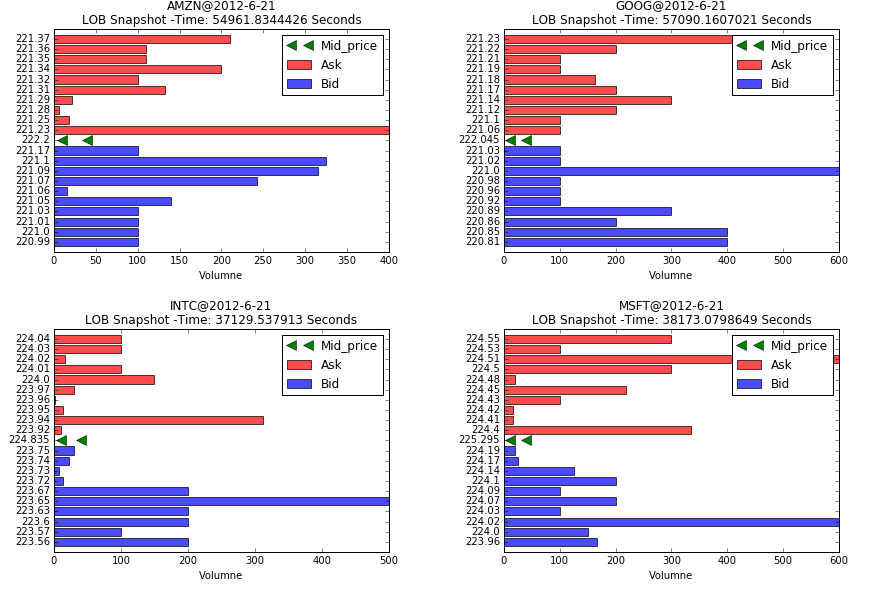
\includegraphics[width=4.5in,  height=3.5in]{figures/snapshot.png}
  \end{center}
\caption{Limit order book examples,   X-axis denotes the volume of each order book and the Y-axis is the price level of each order book,  the left top is AMZN,   the right top is GOOG,   the left bottom is INTC,   and the right bottom is MSFT.Those are snapshots from 2012-06-21} \label{fig:order_snapshot}
\end{figure}

\section{Model framework}
Our model aims to predict the arbitrage opportunities of limit order book price change. There are two kinds of arbitrage in our case: ask price lower arbitrage, denoted by ask-low, and bid price higher arbitrage, denoted by bid-high. We know that at any given time,   the ask price will always higher than the bid price,   so there is no arbitrage. However if the ask price at a future $\Delta t$ time is lower than the current bid price,   then there exists an arbitrage. How to realize it? The arbitrageur can sell short the stock at current bid price $b_t $ and wait for $\Delta t$ time,   buy the stock from the market with the price of ask price $a_{t+\Delta t}$,   and  return the stock required by the short positions,   the profit he can earn without risk is $b_t-a_{t+\Delta t}$. On the bid-high situation,   the arbitrage strategy is similar. Figure \ref{fig:ask_low},   figure \ref{fig:bid_high},   and figure \ref{fig:no_arbi} give us examples of ask-low arbitrage,   bid-high arbitrage,   and no arbitrage cases respectively.

\begin{figure} [hp]
  \begin{center}
    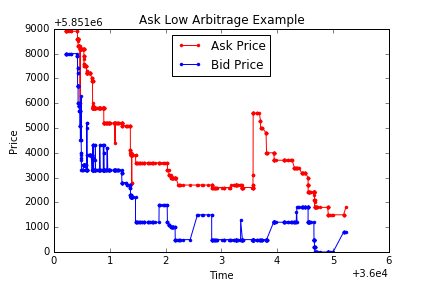
\includegraphics[width=4in,  height=4in]{figures/ask_low_example.png}
  \end{center}
\caption{Ask-low arbitrage example, X-axis represents time in second and Y-axis represents the price times 10000 in dollar, the red line is the ask price and the blue line is the bid price. The ask price after 10 seconds is lower than the current bid price.} \label{fig:ask_low}
\end{figure}


\begin{figure} [hp]
  \begin{center}
    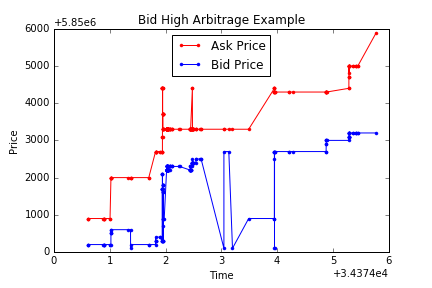
\includegraphics[width=4in,  height=4in]{figures/bid_high_example.png}
  \end{center}
\caption{Bid-high arbitrage example,X-axis represents time in second and Y-axis represents the price times 10000 in dollar, the red line is the ask price and the blue line is the bid price. The bid price after 5 seconds is higher than the current ask price} \label{fig:bid_high}
\end{figure}


\begin{figure} [hp]
  \begin{center}
    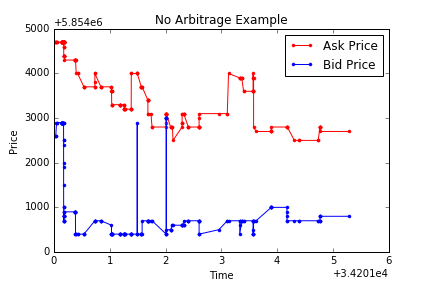
\includegraphics[width=4in,  height=4in]{figures/no_arbi_example.png}
  \end{center}
\caption{No arbitrage example,X-axis represents time in second and Y-axis represents the price times 10000 in dollar, the red line is the ask price and the blue line is the bid price. There is no price spread crossing after 5 seconds.} \label{fig:no_arbi}
\end{figure}

Instead of predicting the price change of future events,   as most past papers did,   we focus on predict the price change in a fixed future time interval,  e.g. 5 seconds later.

\begin{figure} [hp]
  \begin{center}
    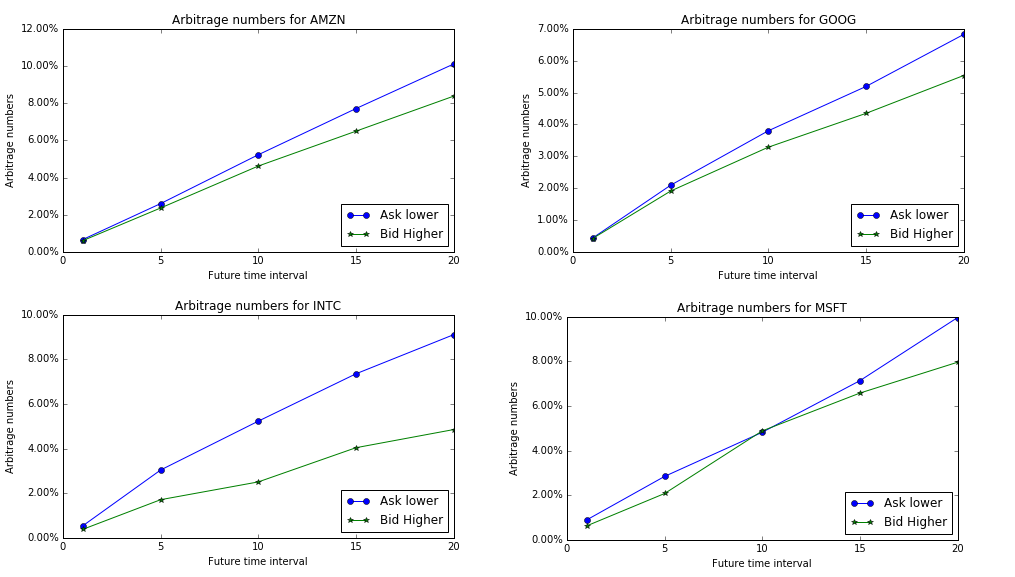
\includegraphics[width=4in,  height=4in]{figures/arbitrage_time.png}
  \end{center}
\caption{Arbitrage numbers based on future time interval, X-axis represents different time intervals and Y-axis is percentage of arbitrage opportunities among all the transactions.Blue line is ask-low cases and green line is bid-high cases} \label{fig:arbitrage_time}
\end{figure}

From figure \ref{fig:arbitrage_time},   we can find that the arbitrage numbers for both bid-high and ask-low opportunities are increasing. For the five seconds time interval,   the percentage of arbitrage opportunities among all the transaction is around 2\% for each stock listed in the figure. For the ten seconds time interval,   the arbitrage percentage increases to around 4\%,   which almost doubled. 

In general,  we need to build different learning models should be built for capturing dynamics of limit order books under different metrics. There are typically four steps to design a machine learning model for a specific
metric.
1) Extracting features: building a suitable format for machine learning schemes to handle by transforming the raw order book data  and message book data.
2) Constructing learning models: building models of AdaBoost and random forest with the given features from step 1. 
3) Validating learning model: Evaluating and validating the model by means of specific performance measurements.
4) Classifying out of sample data: applying the  constructed learning model to forecast the chosen testing set in real time.

\section{Features}
Time intervals between two consecutive events can vary from
milliseconds to several minutes of difference. Event-based data representation
avoids issues related to such big differences in data flow. As a result,   each of
our representations is a vector that contains information for 10 consecutive
events. Event-based data description leads to a dataset of approximately
half a million representations (i.e. 394337 representations). We represent
these events using the 144-dimensional representation proposed recently by
\cite{kercheval2015modelling}  ,   formed by three types of features: a) the raw
data of a ten-level limit order containing price and volume values for bid
and ask orders,   b) features describing the state of the LOB exploiting past
information and c) features describing the information edge in the raw data
by taking time into account. Derivation of time,   stock price and volume are
calculated for short and long term projection. Particularly,   types in features
$v_7$ ,   $v_8$ and $v_9$ are: trades,   orders,   cancellations,   deletion,   execution of a visible
limit order and execution of a hidden limit order respectively. The features are listed in the following figure and can be referred in \cite{kercheval2015modelling},   details can be found in table \ref{tab:features}. 

\begin{table}
   	\caption{Featur\label{key}es summary,   nine datasets including basic set,   time insensitive set,   and time sensitive set,   totally 156 features}
   	\label{tab:features}
   	\begin{center} 
   	\scalebox{0.8}{
   		\begin{tabular}{|l|l| }
   			\hline
   			Basic Set & Description(i=level index,  n=10)\\[5pt]
   			\hline 
   			
   			$v_1=\{P_i^{ask},  V_i^{ask},  P_i^{bid},  V_i^{bid}\}_{i=1}^n$   & price\ and\ volume(n levels)\\[5pt]
   			\hline
            Time-insensitive Set & Description(i=level index)\\[5pt]
   			\hline 
   			$v_2=\{(P_i^{ask}-P_i^{bid}),  (P_i^{ask}+P_i^{bid})/2\}_{i=1}^n$   & bid ask spreads and mid prices(n levels)\\[5pt]
   			
   			$v_3=\{|P_{i+1}^{ask}-P_1^{ask}|,  (P_{i+1}^{bid}-P_1^{bid}|,  |P_{i+1}^{ask}-P_i^{ask}|,  |P_{i+1}^{bid}-P_i^{bid}|\}_{i=1}^{n-1}$ & price difference\\[5pt]
   			
   			$v_4=\{\frac{1}{n}\sum_{i=1}^n P_i^{ask},  \frac{1}{n}\sum_{i=1}^n P_i^{bid},  \frac{1}{n}\sum_{i=1}^n V_i^{ask},  \frac{1}{n}\sum_{i=1}^n V_i^{bid} \}$& mean prices and volumes\\[5pt]
   			
   			$v_5=\{\sum_{i=1}^{n}(P_i^{ask}-P_i^{bid}),  \sum_{i=1}^{n}(V_i^{ask}-V_i^{bid})\}$   & accumulated difference\\[5pt]
				
				\hline
		   Time-sensitive Set & Description(i=level index)\\[5pt]
		   \hline
		   
		   $v_6=\{\partial P_i^{ask}/\partial t,  \partial P_i^{bid}/\partial t,  \partial V_i^{ask}/\partial t,  \partial V_i^{bid}/\partial t \}_{i=1}^n$ & price and volume derivatives\\
		   
		    $v_7=\{\lambda_{\Delta_t}^{la},  \lambda_{\Delta_t}^{lb},  \lambda_{\Delta_t}^{ma},  \lambda_{\Delta_t}^{mb},  \lambda_{\Delta_t}^{ca},  \lambda_{\Delta_t}^{cb}\}$& average intensity of each type\\
		    
		     $v_8=\{1_{\lambda_{\Delta_t}^{la}>\lambda_{\Delta_T}^{la}},  1_{\lambda_{\Delta_t}^{lb}>\lambda_{\Delta_T}^{lb}},  1_{\lambda_{\Delta_t}^{ma}>\lambda_{\Delta_T}^{ma}},  1_{\lambda_{\Delta_t}^{mb}>\lambda_{\Delta_T}^{mb}}\}$& relative intensity indicators\\
		     
		   $v_9=\{\partial \lambda^{ma}/\partial t,  \partial \lambda^{lb}/\partial t,  \partial \lambda^{mb}/\partial t,  \partial \lambda^{la}/\partial t$ \} & accelerations(/limit) \\
		   \hline		    
   		\end{tabular}
   		}
   	\end{center}
\end{table} 


\section{Model measurement and numerical results}
As we mentioned before,   the arbitrage opportunities are rare events among all the placement of order books. For example,   the percentages of arbitrage opportunities of five seconds interval is only around 2 \%,   so the accuracy rate of a model is not a good measurement.  Because if we define all the results of a testing sample as no arbitrage,   we can still get a very high accuracy rate,   which is around 98 \%. Therefore we introduce precision,   recall and f1 score to deal with this problem. \\
Some terms here:\\
Positive (P): Observation is positive.   In our case,   it means that arbitrage opportunity will occur in the future.\\
Negative (N): Observation is negation.   In our case, it means that there is no arbitrage in the future. \\
True positive(TP): Observation is positive and is classified as positive.   In our case, it means that the detected arbitrage opportunity is a real arbitrage opportunity.\\
False negative(FN):Observation is positive but is classified as negative,  in our case, we do not detect a real arbitrage opportunity\\
True negative(TN): Observation is negative and is classified as negative,  in our case, it means the detected no arbitrage case is actually no arbitrage\\
False positive(FP): Observation is negative but is classified as positive,  in our case, it means that the detected arbitrage case is actually no arbitrage. \\
The precision is: \\
\begin{equation}
Precision=\frac{TP}{TP+FP}=\frac{positive\ predicted\ correctly}{all\ positive\ predictions}
\end{equation} 
The recall is:\\
\begin{equation}
Recall=\frac{TP}{TP+FN}=\frac{positive\ predicted\ correctly}{all\ positive\ observations}
\end{equation} 
F1 score:\\
\begin{equation}\label{eg:f1}
F_1=2\frac{Precision*Recall}{Precision+Recall}
\end{equation} 
From equation \ref{eg:f1},   $F1$ score is the harmonic mean of precision and recall\\ 
Table \ref{tab:ask_low_prediction} shows the results of predicting ask-lower opportunity of stock AMZN.
\begin{table} [hp]
	\caption{AMZN ask-low arbitrage opportunities prediction(5 seconds)}
	\label{tab:ask_low_prediction}
	\begin{center}
	\scalebox{0.8}{
		\begin{tabular}{|c|c|c|c|c|c|c|}
			\hline
			 Model& Training & Training  & Test  & Test & Test & Test \\[5pt]
			 & time(s) & F1 score & time(s) & Recall & Precision & F1 score \\[5pt]
			 \hline
			 Logistic regression(Lasso penalty)& 260.7 & 8.8 \% & 0.002 & 2.9\% & 75.0\%& 5.6\%\\[5pt]
			 Logistic regression(Ridge penalty)& 7.2 & 8.8 \% & 0.01 &  2.9\% & 75.0\%& 5.6\%\\[5pt]
			 SVM(Poly 2 kernal,  5000 estimator)& 75.7 & 61.5 \% & 4.3 &  29.1\% & 96.8\%& 44.8\%\\[5pt]
			 Decision Tree(no pruning)& 3.9 & 61.8 \% & 0.003 &  30.1\% & 91.2\%& 45.3\%\\[5pt]
			 AdaBoost(number of estimate=100)& 30.0 & 96.5 \% & 0.04 & 73.8 \% & 92.7\% &  82.2\% \\[5pt]
			 Random forest(number of estimate=100)& 37.5 & 99.1 \% & 0.11 & 72.8 \% & 96.2\% &  82.9\% \\[5pt]		 	
	 		\hline 
		\end{tabular}
		}
	\end{center}
\end{table}
 
Here the number of training samples is 90000 and the number of testing samples are 10000. Computer has 8G memory and Intel Xeon E3 processor. The results for other stocks can be found in Appendix A\\

\section{Multiclass prediction problem}

There are three cases of arbitrage opportunities in our research including ask-low, bid-high,  and no arbitrage. If we want to predict these three cases at the same time,  then our model is transformed into a multi-category classification problem. For this kind of problem,  we focus on learning a predictor $h:\mathcal{X}\rightarrow \mathcal{Y}$,  where $\mathcal{Y}$ represents a set of categories and $\mathcal{X}$ is the set of independent variables. The most widely accepted way that deals with the multiclass learning problem,  is to reduce the multiclass classification to binary classification.  Two straightforward methods,  one vs. rest and one vs. one,  are introduced in the following:

In the one vs. rest method,   we train $k$ binary classifiers,  where $k$ is the number of classes for response $y$. Each binary classifier distinguishes the dependent variable $y$ between one class and the rest of the other classes.  More clearly,   given a training set  $S=(x_1, y_1), ...,  (x_m, y_m)$,  where each $y_i$ is in $\mathcal{Y}$ and $m$ is the amount of data sample,  we build $k$ binary training sets,  $S_1, ..., S_k$,  where $S_i=(x_1, (-1)^{\mathds{1}_[y_1\neq i]}), ..., (x_m, (-1)^{\mathds{1}_[y_m\neq i]}).$ In word description,  
$S_i$ is the set of data labeled 1 if their class is i,  and -1 otherwise. For each $i \in [k]$,  we train a binary predictor $h_i:\mathcal{X}\rightarrow \{+1, -1\}$ based on $S_i$ and expect that the result of $h_i(x)$ will equal to 1 if and only if $x$ is in class $i$.  Therefore,  given $h_1, ..., h_k$,  we build a multiclass predictor using the principle: 
\begin{equation}
h(x) \in\underset{i\in [k]}{\operatorname{argmax}}\ h_i(x)
\end{equation}
When there are more than one predictors that predict ``1",  we can break the ties by choosing the minimal index in $argmax_i h_i(x)$. The description of the one vs.rest method is given in algorithm \ref{alg:onevsrest}.


\begin{algorithm}[H]
	\caption{One vs. rest algorithm, }  \label{alg:onevsrest}
	\nl \textbf{Input:}\;
	\nl training set $S=(x_1, y_1), ..., (x_m, y_m)$\;
	    algorithm for binary classification $A$\;
	
	\For{$i\in \mathcal{Y}$}{
		\nl let $S_i=(x_1, (-1)^{\mathds{1}_[y_1\neq i]}), ..., (x_m, (-1)^{\mathds{1}_[y_m\neq i]}).$ \;
		\nl let $h_i=A(S_i)$ \;		
	}
	\nl \textbf{Output:} \;
	the multiclass hypothesis defined by $h(x)\in  \underset{i\in \mathcal{Y}}{\operatorname{argmax}}\ h_i(x)$\;
\end{algorithm}


Another widely used multiclass approach is one vs. one,  which compares all pairs of classes with each other. That is,  given a training set $S=(x_1, y_1), ..., (x_m, y_m)$,  where every $y_i$ is in $[k]$,  we build a binary training sequence,  $S_{ij}$,  for every $1\leq i <j\leq k$. The set $S_{ij}$ include all instances from $S$ whose label is either $i$ or $j$. In each $S_{ij}$,  we set the label of $S_{ij}$ as +1 if the class label in $S$ is $i$ and -1 if the class label in $S$ is $j$. Wo conduct the same process on every $S_{ij}$ to get a multiclass classifier $h_{ij}$. The final result of the multiclass classifier is obtained by a highest number of ''wins". The description of the one vs. one method is given in algorithm \ref{alg:onevsone}:


\begin{algorithm}[H]
	\caption{One vs. one method}\label{alg:onevsone}
	\nl \textbf{Input:}\\
	\nl Training set $S=(x_1, y_1), ..., (x_m, y_m)$\;
	Algorithm for binary classification $A$\;
	\nl \For{each $i, j$ in $\mathcal{Y}$,  such that $i<j$}{
		Initialize $S_{ij}$ to be the empty sequence\;
		\nl \For{$t=1, ..., m$}{
			\nl	If $y_t=i$ add (x_t, +1)\ to\ $S_{ij}$\;
			\nl	If $y_t=j$ add (x_t, -1)\ to\ $S_{ij}$\;
			
		}
		\nl Let $h_{ij}=A(S_{ij})$\;		
	}
	\nl	\textbf{Output:}\\
	\nl	The multiclass hypothesis defined by 
	$h(x) \in argmax_{i \in \mathcal{Y}}(\sum_{j\in \mathcal{Y}}sign(j-i)h_{ij}(x))$ \;
	
\end{algorithm} 


\begin{figure} [hp]
	\begin{center}
		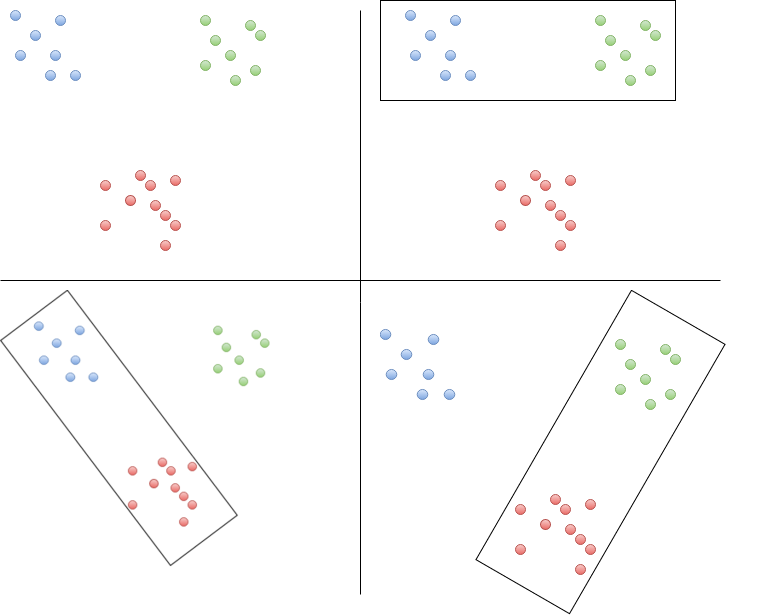
\includegraphics[width=4in,  height=4in]{figures/onevsone.png}
	\end{center}
	\caption{One vs. one algorithm,  the upper left figure shows the original three classes(represent as red,  green,  and blue),  the upper right figure only considers blue and green classes,  the bottom left figure only considers blue and red classes,  and bottom right figure only considers red and green classes. } \label{fig:onevsone}
\end{figure}

\begin{figure} [hp]
	\begin{center}
		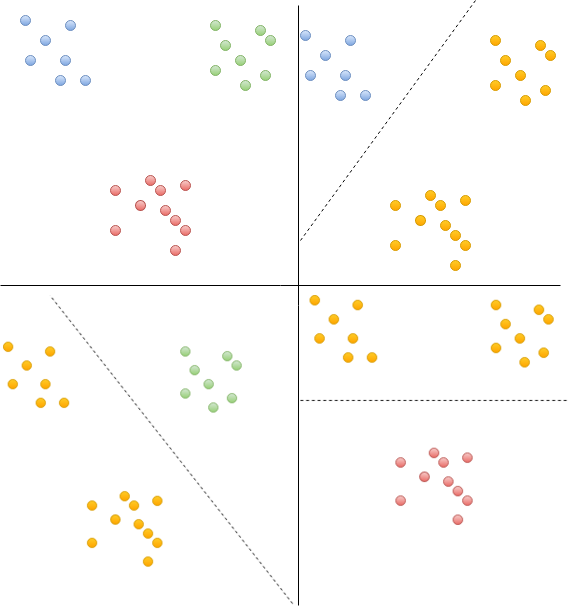
\includegraphics[width=4in,  height=4in]{figures/onevsrest.png}
	\end{center}
	\caption{One vs. rest algorithm, the upper left figure shows the original three classes(represent as red,  green,  and blue), the upper right figure considers blue and the rest classes, the bottom left figure considers green and the rest classes,  and bottom right figure considers red and the rest classes. } \label{fig:onevsrest}
\end{figure}


\section{Feature importance}
In statistical and machine learning area,   feature and variable selection play a very important role. There are some benefits of the feature selection to researchers: 1) It can improve the prediction performance of the predictors. 2) The predictors can be faster and more cost-efficiency. 3) It help people to better understand the meaning hidden behind models to generate the data.  
\cite{breiman2001random} proposes a formula to evaluate the importance of a variable $X_m$ for predicting $Y$ by adding up the weighted impurity decreases $p(t)\Delta_i(s_t,  t)$ for all nodes $t$ where $X_m$ is used,   averaged over all $N_T$ trees in the forest:
\begin{equation}\label{eq:importance}
\begin{aligned}
Imp(X_m)=\frac{1}{N_T}\sum_T\sum_{t\in T:v(s_t)=X_m}p(t)\Delta_i(s_t,  t)\\
\\
\Delta_i(s,t)=i(t)-p_Li(t_l)-p_Ri(t_R)
\end{aligned}
\end{equation}
where $i(t)$ is a given impurity measure, $p(t)$ is the proportion $N_t/N$ of samples reaching $t$ , $v(s_t)$ is the variable used in split $s_t$, $p_L=N_{t_L}/N_t$ and $p_R=N_{t_R}/N_t$. The equation \ref{eq:importance} is referred as \textit{Mean Decrease Impurity importance} (MDI). Figure \ref{fig:feature_importance} and table \ref{tab:feature_importance} show the results of feature importance of the four stocks based on random forest models. We find that feature importance varies from stock to stock,   there is no obvious rule according to it. To look more closely,   we list the top 3 features for each stock. For stock AMZN,   the first three important features are 107,   106 and 116 which represents $\partial P_5^{ask}/\partial t$,   $\partial P_6^{ask}/\partial t$,   and $\partial P_4^{bid}/\partial t$ respectively. The first 3 import stock for GOOS are 41,  3,  51 which represent $P_1^{ask}-P_1^{bid}$,   $P_3^{ask}$,   and $P_1^{ask}+P_1^{bid}$. For stock INTC,   they are 16,  36,  40 which represents $V_6^{ask},  V_6^{bid}$,   and $V_{10}^{bid}$. For stock MSFT,   they are 28,  12 and 16 which represent $P_8^{bid},  V_2^{ask}$,   and $V_6^{ask}$. We can see that the derivative of price to time is important to stock AMZN. For stock GOOG,   the relationship of bid price and ask price becomes more important. Ask volume and bid volume are essential for stock INTC,   price and volume are critical to stock MSFT.   


\begin{table}[hp]
	\caption{Feature importance based on random forest model}
	\label{tab:feature_importance}
	\begin{center}
	\rotatebox{270}{
		\begin{tabular}{cccccccc}
		\hline
			\multicolumn{2}{c}{ AMZN} & \multicolumn{2}{c}{GOOG}& \multicolumn{2}{c}{INTC}& \multicolumn{2}{c}{MSFT}\\
			\hline
			 Feature index  &  Importance& Feature index  &  Importance &Feature index  &  Importance & Feature index  &  Importance\\
			 \hline
		107& 3.997699& 41& 2.497344& 16& 4.930035& 28& 3.777894\\
		108& 2.531017& 3& 2.077711& 36& 3.584072& 12& 3.668482\\
		116& 1.72645& 51& 1.911522& 40& 3.271213& 16& 3.462065\\
		12& 1.523849& 71& 1.860316& 14& 2.930865& 36& 3.307528\\
		41& 1.489288& 111& 1.7199& 30& 2.830366& 8& 3.134871\\
		52& 1.401763& 70& 1.511696& 20& 2.694488& 26& 2.863927\\
		61& 1.390584& 82& 1.503223& 22& 2.594267& 30& 2.783838\\
		51& 1.296778& 42& 1.476138& 38& 2.575397& 20& 2.782014\\
		1& 1.26687& 7& 1.446197& 28& 2.565284& 24& 2.752804\\
		81& 1.24307& 52& 1.413531& 32& 2.510037& 32& 2.722132\\
		3& 1.240166& 53& 1.410323& 18& 2.485869& 38& 2.660868\\
		9& 1.222178& 80& 1.379994& 24& 2.388528& 81& 2.45301\\
		79& 1.187279& 8& 1.3286& 82& 2.289012& 82& 2.312318\\
		80& 1.168383& 84& 1.316409& 12& 2.165716& 40& 2.276727\\
		53& 1.16105& 24& 1.246773& 26& 2.119569& 34& 2.149401\\
		54& 1.150503& 15& 1.223152& 4& 2.032679& 10& 1.790342\\
		82& 1.150272& 55& 1.214248& 8& 2.007556& 18& 1.765228\\
		118& 1.133169& 16& 1.211959& 34& 1.950585& 14& 1.727172\\
		7& 1.131877& 57& 1.199527& 81& 1.896318& 22& 1.649081\\
		84& 1.099623& 1& 1.178082& 6& 1.697322& 84& 1.515854\\
\hline 
		\end{tabular}
		}
	\end{center}
\end{table}


\begin{figure} [hp]
  \begin{center}
    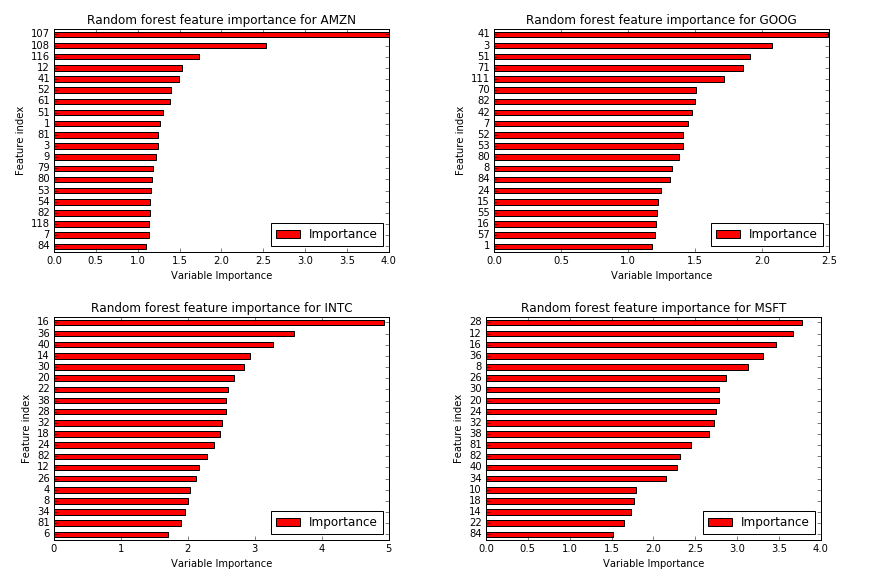
\includegraphics[width=6in,  height=5in]{figures/feature_importance.png}
  \end{center}
\caption{Feature importance. X-axis is the feature importance and Y-axis is the corresponding feature index.The top left panel shows the result of AMZN,   the top right panel shows the result of GOOG,  the bottom left panel shows the result of INTC,   and the bottom right panel shows the result of MSFT. } \label{fig:feature_importance}

\end{figure}
Since the numbers of features in bid side and in ask side are equal, we count the numbers of features among top 20 important features to see which side is more important. For mid prices and bid ask spread features, we count on both bid and ask side. From the results of table \ref{tab:feature_importance_ask_bid}, we can see that features on ask side play a more important role. It may be caused by the fact that we observe the ask low case in this experiment. 
	\begin{table}[hp]
		\caption{Ratio of features on bid and ask side }
		\begin{center}
			\scalebox{0.8}{
				\begin{tabular}{| c | c|c|c|c|}
					\hline
					Side  &AMZN &GOOG & INTC & MSFT \\
					\hline 
					Ask side features & 18& 17 &10 &10\\
					Bid side features & 7& 10 &10 &10\\
					Ratio of ask to bid &2.6 &1.7&1 &1\\
					\hline	 	
				\end{tabular}
			}
		\end{center}
	\end{table}

Table \ref{tab:feature_importance_occurrence} shows the most frequent occurrence features among four stocks. We find that price differences between adjacent price level are important.
	\begin{table}[hp]
		\caption{The most frequent occurrence features among four stocks}
		\label{tab:feature_importance_occurrence}
		\begin{center}
			\scalebox{0.8}{
				\begin{tabular}{| c | c|c|c|c|}
					\hline
					Index  & Feature & Number of occurrence \\
					\hline
					82 & $|p_5^{ask}-P_4^{ask}|$ & 4\\
					84 & $|p_7^{ask}-P_6^{ask}|$& 3\\
					81 & $|p_4^{ask}-P_3^{ask}|$& 3\\
					24 & $p_4^{bid}$& 3\\
					16 & $V_6^{ask}$& 3\\
					12 & $ V_2^{ask}$& 3\\
					8 & $ P_8^{ask}$& 3\\
					\hline	 	
				\end{tabular}
			}
		\end{center}
	\end{table}


\section{Trading strategy}
There are some measurements to test the performance of trading strategy,   in our research we choose the Profit-and-Loss(PnL). 
According to \cite{zhou2015evolution},  suppose we have $y_t=S_{t+H}-S_t$ as the price change from time $t$ to $t+H$,   and $\hat{y_t}$ as the prediction result of our model,   $c$ is the trading cost. Assume that we will make a trading decision if the profit is bigger than a significant level,   $\hat{y_t}>\alpha$,   or conversely,   the loss is bigger than a significant level,  $\hat{y_t}<-\alpha$.The PnL within the time interval $[t,  t+H]$ is the profit and loss through a transaction which can be written as follows:\\
\begin{equation}       
PnL=\left\{          
  \begin{array}{ll}   
    y-c  & y>=\alpha,   buy\ action   \\  
     -y-c & y<=-\alpha,   sell\ short\ action \\
     0 & otherwise
  \end{array}
\right.       
\end{equation}
where y is the net capital gain from a transaction,   $\alpha$ is significant level and $c$ is the trading cost. The liquidity of taking the orders and information acquisition usually influence the trading cost. In addition, when a large number of volumes come to the market,   the trading cost tends to increases. The stocks that we studied are all big information technology companies,   so the liquidity of those companies is relatively high. Usually,   the trading cost of liquid products is low than one bid-ask spread,   which is around \$0.02 per trade on NASDAQ. Therefore it is feasible that we assume our trading cost is \$0.02.
In the following,  we define a simple buy-low and sell-high strategy. The details are in algorithm \ref{alg:trading_algorithm}


\begin{algorithm} [hp]
\caption{Naive trading algorithm,  }\label{alg:trading_algorithm}

				         		    \nl initialize: PnL=0\\				         		    
				         		    \nl \For{i =1 to length(test\_set)}{
				         		    \nl input test\_set[i] features into model and get result of Predict[i]\\
				         		    \nl \If{Predict[i]==1(Ask low)}{
				         		         Sell short at bid price\\
				         		         Clear the short option $\Delta t$ seconds later\\
				         		         PnL+=$Bid\_price_{t}-Ask\_price_{t+\Delta t}-cost$}
				         		        \ElseIf{Predicted[i]==-1(Bid high)}
				         		         {Buy at ask price\\
				         		         Sell at bid price $\Delta t$ seconds later\\
				         		          PnL+=$Bid\_price_{t+\Delta t}-Ask\_price_t-cost$}\\
				         		        \Else
				         		         {Take no action} \\
				         		    \nl  \Return PnL 
				         		     }				  				         		    
			\end{algorithm} \\			


\begin{figure} [hp]
  \begin{center}
    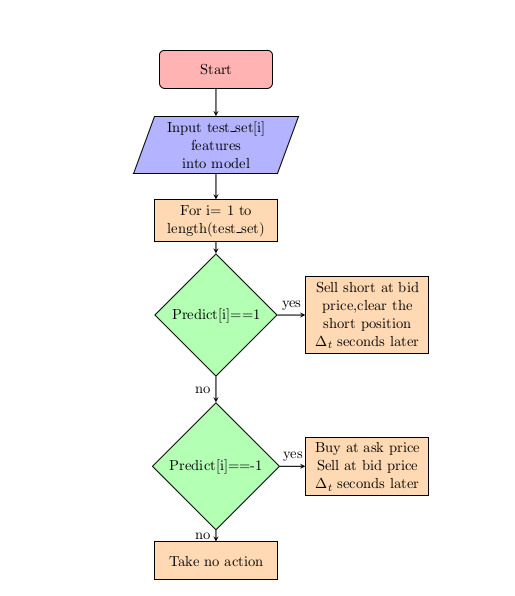
\includegraphics[width=6in,  height=6in]{figures/strategy_algorithm.png}
  \end{center}
\caption{Naive trading strategy framework. When the ask-low cases (prediction result as 1) occur,   we can sell short at the current bid price and buy the stock back at the future ask price. Similarly,   when the bid-high cases (prediction result as -1) occurs,   we can buy the stock at the current ask price and sell the stock to the market at the future bid price. } \label{fig:strategy_algorithm}
\end{figure}


Figure \ref{fig:strategy_algorithm} gives us an example of how to conduct a naive arbitrage trading,   when the ask-low cases (green triangles)  occur,   we can sell short at the current bid price and buy the stock back at the future ask price. Similarly,   when the bid-high cases (red triangles) occurs,   we can buy the stock at the current ask price and sell the stock to the market at the future bid price. 

In the following, we show the results of prediction results of stock AMZN,   random forest and AdaBoost methods are used. Additionally,   for multi-class problems,   one vs. one and one vs. rest methods are utilized. 

Prediction results of random forest one vs. one method for stock AMZN:\\
\begin{center}
$\left [{\begin{array}{*{20}c}
109    & 27  & 0 \\
  0  & 9736 & 3 \\
  0 & 33 & 92

 \end{array} } \right]
$ 
\end{center}
\\


Prediction results of random forest one vs rest method for stock AMZN:\\
\begin{center}
$\left [{\begin{array}{*{20}c}
109    & 27  & 0 \\
  0  & 9737 & 2 \\
  0 & 38 & 87

 \end{array} } \right]
$ 
\end{center}
\\

Prediction results of AdaBoost one vs one method for stock AMZN:\\
\begin{center}
$\left [{\begin{array}{*{20}c}
128    & 8  & 0 \\
  2  & 9726 & 11 \\
  0 & 18 & 107

 \end{array} } \right]
$ 
\end{center}
\\

Prediction results of AdaBoost one vs rest method for stock AMZN:\\
\begin{center}
$\left [{\begin{array}{*{20}c}
120    & 16  & 0 \\
  0  & 9736 & 3 \\
  0 & 27 & 98
 \end{array} } \right]
$ 
\end{center}
\\
\\
Visualized confusion matrix can be found in figure \ref{fig:amzn_confusion_matrix}. More results for all stocks are listed in appendix A.

\begin{figure} [hp]
  \begin{center}
    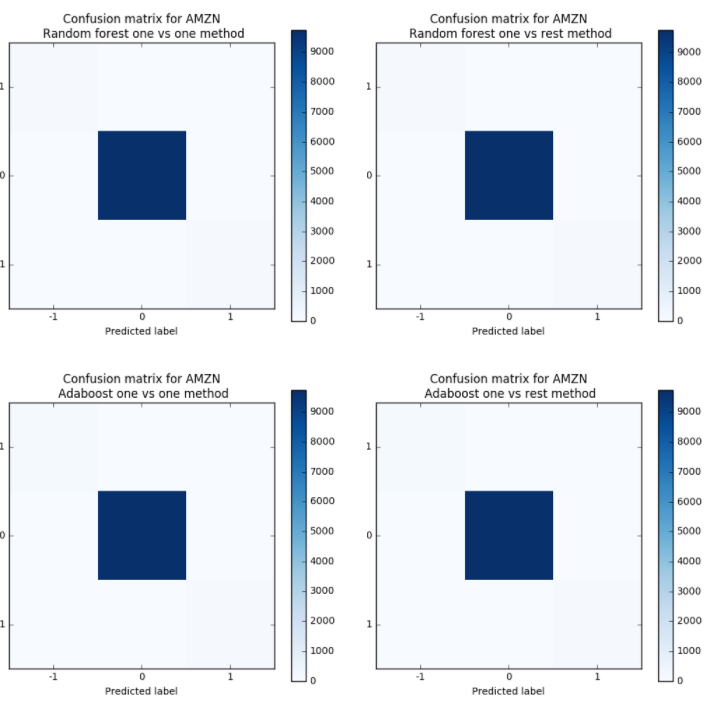
\includegraphics[width=6in,  height=6in]{figures/amzn_confusion_matrix.png}
  \end{center}
\caption{Confusion matrix of stock AMZN,   -1 represents bid-high arbitrage,   1 represents ask-low arbitrage and 0 means no arbitrage. X-axis is the predicted label and Y-axis is the true label} \label{fig:amzn_confusion_matrix}
\end{figure}


Figure \ref{fig:amzn_pnl} shows the PnL for stock AMZN under random forest and AdaBoost methods. The red dots represent the bid-high cases and the blue dots represent the ask-low cases. If the dot lies above the X-axis,  it means that this transaction will earn money and vice versa. The trading cost is \$0.02,   and we can see that most transactions are profitable. From figure \ref{fig:amzn_cum_pnl} we can find that our cumulative PnL shows a very good performance of our trading strategy. One reason to explain this is that our model returns a very good precision score. We will take action if our prediction result is non-zero,   so high precision is very helpful. If our model predicts no arbitrage,   then we will take no action,   so misclassifying of an arbitrage case to a nonarbitrage case will not impact our profitability. Therefore,   the recall score is not as important as the precision score in our strategy. The PnL results for other stocks are listed in the appendix A. 

\begin{figure} [hp]
  \begin{center}
    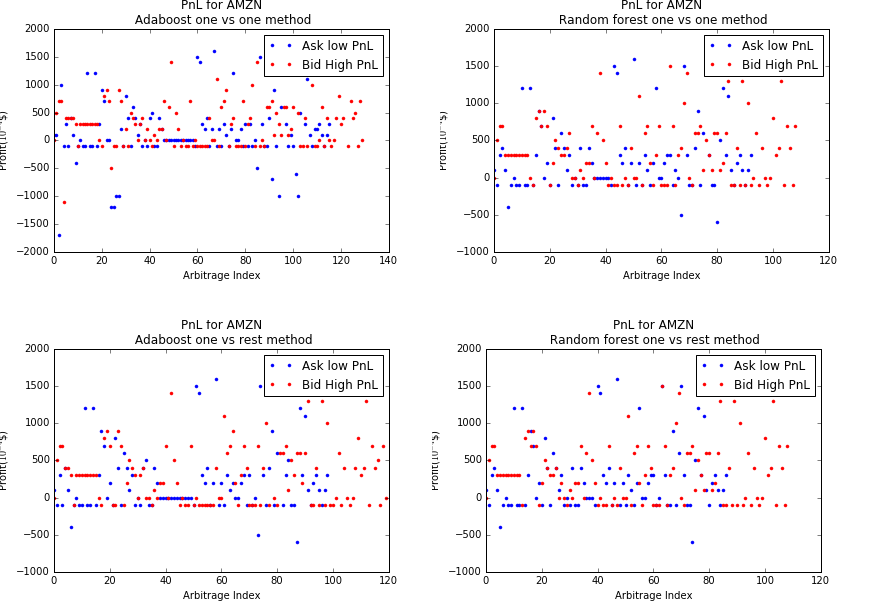
\includegraphics[width=6in,  height=5in]{figures/amzn_pnl.png}
  \end{center}
\caption{PnL for AMAN based on random forest and AdaBoost methods,    X-axis represents the predicted arbitrage index and Y-axis is profit or loss for each transaction.The top left panel shows the result of AdaBoost one vs. one method,   the top right panel shows the result of random forest one vs. one method,  the bottom left panel shows the result of AdaBoost one vs. rest method,   and the bottom right panel shows the result of random forest one vs. rest method. Trading cost is \$0.02} \label{fig:amzn_pnl}
\end{figure}

\begin{figure} [hp]
  \begin{center}
    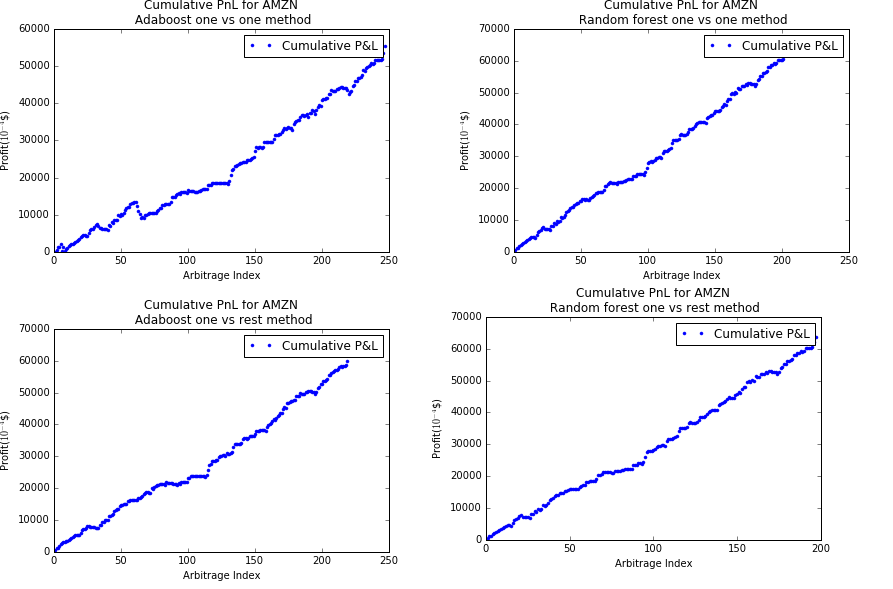
\includegraphics[width=6in,  height=5in]{figures/amzn_cum_pnl.png}
  \end{center}
\caption{Cumulated PnL for AMAN based on random forest and AdaBoost methods,    X-axis represents the predicted arbitrage index and Y-axis is profit or loss for each transaction.The top left panel shows the result of AdaBoost one vs. one method,   the top right panel shows the result of random forest one vs. one method,  the bottom left panel shows the result of AdaBoost one vs. rest method,   and the bottom right panel shows the result of random forest one vs. rest method. Trading cost is \$0.02} \label{fig:amzn_cum_pnl}
\end{figure}
